\documentclass[ignorenonframetext,]{beamer}
\usetheme{default}
\usecolortheme{rose}
\usepackage{amssymb,amsmath}
\usepackage{ifxetex,ifluatex}
\usepackage{fixltx2e} % provides \textsubscript
\ifxetex
  \usepackage{fontspec,xltxtra,xunicode}
  \defaultfontfeatures{Mapping=tex-text,Scale=MatchLowercase}
\else
  \ifluatex
    \usepackage{fontspec}
    \defaultfontfeatures{Mapping=tex-text,Scale=MatchLowercase}
  \else
    \usepackage[utf8]{inputenc}
  \fi
\fi
\usepackage{color}
\usepackage{fancyvrb}
\DefineShortVerb[commandchars=\\\{\}]{\|}
\DefineVerbatimEnvironment{Highlighting}{Verbatim}{commandchars=\\\{\}}
% Add ',fontsize=\small' for more characters per line
\newenvironment{Shaded}{}{}
\newcommand{\KeywordTok}[1]{\textcolor[rgb]{0.00,0.44,0.13}{\textbf{{#1}}}}
\newcommand{\DataTypeTok}[1]{\textcolor[rgb]{0.56,0.13,0.00}{{#1}}}
\newcommand{\DecValTok}[1]{\textcolor[rgb]{0.25,0.63,0.44}{{#1}}}
\newcommand{\BaseNTok}[1]{\textcolor[rgb]{0.25,0.63,0.44}{{#1}}}
\newcommand{\FloatTok}[1]{\textcolor[rgb]{0.25,0.63,0.44}{{#1}}}
\newcommand{\CharTok}[1]{\textcolor[rgb]{0.25,0.44,0.63}{{#1}}}
\newcommand{\StringTok}[1]{\textcolor[rgb]{0.25,0.44,0.63}{{#1}}}
\newcommand{\CommentTok}[1]{\textcolor[rgb]{0.38,0.63,0.69}{\textit{{#1}}}}
\newcommand{\OtherTok}[1]{\textcolor[rgb]{0.00,0.44,0.13}{{#1}}}
\newcommand{\AlertTok}[1]{\textcolor[rgb]{1.00,0.00,0.00}{\textbf{{#1}}}}
\newcommand{\FunctionTok}[1]{\textcolor[rgb]{0.02,0.16,0.49}{{#1}}}
\newcommand{\RegionMarkerTok}[1]{{#1}}
\newcommand{\ErrorTok}[1]{\textcolor[rgb]{1.00,0.00,0.00}{\textbf{{#1}}}}
\newcommand{\NormalTok}[1]{{#1}}
\usepackage{url}
% Comment these out if you don't want a slide with just the
% part/section/subsection/subsubsection title:
\AtBeginPart{\frame{\partpage}}
\AtBeginSection{\frame{\sectionpage}}
\AtBeginSubsection{\frame{\subsectionpage}}
\AtBeginSubsubsection{\frame{\subsubsectionpage}}
\setlength{\parindent}{0pt}
\setlength{\parskip}{6pt plus 2pt minus 1pt}
\setlength{\emergencystretch}{3em}  % prevent overfull lines
\setcounter{secnumdepth}{0}

\title{Processing 1 - Introduction}
\author{Alex McLean}

\begin{document}
\frame{\titlepage}

\begin{frame}\frametitle{Processing}


\includegraphics[width=0.1\textwidth]{../images/processing2-logo.jpg}

\begin{itemize}
\item
  Free/open source project
\item
  Initiated by Casey Reas and Ben Fry in 2005
\item
  For learning programming in visual context
\item
  Based on Java, but simplified
\item
  Sketchbook metaphor
\end{itemize}

\end{frame}

\begin{frame}\frametitle{On-line documentation}

\begin{center}

\includegraphics[width=0.5\textwidth]{../images/processingorg.png}

\url{https://processing.org/}
\end{center}

\begin{itemize}
\item
  Reference, Tutorials, Forum
\item
  Off-line from UI:

  \begin{itemize}
  \item
    Help -\textgreater{} reference
  \item
    Right click on code -\textgreater{} find in reference
  \end{itemize}
\end{itemize}

\end{frame}

\begin{frame}[fragile]\frametitle{Further reading}


\includegraphics[width=0.5\textwidth]{../images/learningprocessing.jpg}

Video lectures: \url{http://icm.shiffman.net/}

\end{frame}

\begin{frame}\frametitle{Open processing}

\begin{center}

\includegraphics[width=0.5\textwidth]{../images/processingorg.png}

\url{https://openprocessing.org/}
\end{center}

\end{frame}

\begin{frame}\frametitle{Examples}

File -\textgreater{} Examples

\begin{center}
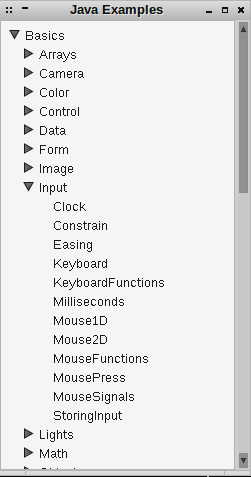
\includegraphics[width=0.3\textwidth]{../images/examples.png}
\end{center}

\end{frame}

\begin{frame}\frametitle{Lets get programming}

\begin{itemize}
\item
  Draw a circle
\item
  Play a sound
\end{itemize}

\end{frame}

\begin{frame}[fragile]\frametitle{Draw a circle}

Use the \texttt{ellipse} function call

Reference:
\href{http://processing.org/reference/ellipse\_.html}{Ellipse}

\begin{Shaded}
\begin{Highlighting}[]
\CommentTok{// x, y, width, height}
\FunctionTok{ellipse}\NormalTok{(}\DecValTok{10}\NormalTok{,}\DecValTok{10}\NormalTok{,}\DecValTok{10}\NormalTok{,}\DecValTok{10}\NormalTok{);}
\end{Highlighting}
\end{Shaded}

Understand:

\begin{itemize}
\item
  Cartesian coordinates and origins
\item
  \url{http://processing.org/tutorials/drawing/}
\end{itemize}

\end{frame}

\begin{frame}\frametitle{Make a sound}

Add the minim library to your sketch.

\end{frame}

\begin{frame}[fragile]\frametitle{Draw ten circles}

In different positions, using copy and paste

\begin{Shaded}
\begin{Highlighting}[]
\FunctionTok{ellipse}\NormalTok{(}\DecValTok{10}\NormalTok{,}\DecValTok{10}\NormalTok{,}\DecValTok{10}\NormalTok{,}\DecValTok{10}\NormalTok{);}
\FunctionTok{ellipse}\NormalTok{(}\DecValTok{20}\NormalTok{,}\DecValTok{20}\NormalTok{,}\DecValTok{10}\NormalTok{,}\DecValTok{10}\NormalTok{);}
\FunctionTok{ellipse}\NormalTok{(}\DecValTok{30}\NormalTok{,}\DecValTok{30}\NormalTok{,}\DecValTok{10}\NormalTok{,}\DecValTok{10}\NormalTok{);}
\end{Highlighting}
\end{Shaded}

and so on\ldots{}

\end{frame}

\begin{frame}[fragile]\frametitle{Draw a hundred circles}

Time to use variables and loops.

\begin{Shaded}
\begin{Highlighting}[]
\CommentTok{// Initialise variable, this will be our loop counter}
\DataTypeTok{int} \NormalTok{i = }\DecValTok{0}\NormalTok{;}

\CommentTok{// repeat until test fails}
\KeywordTok{while} \NormalTok{(i < }\DecValTok{100}\NormalTok{) \{}
  \FunctionTok{ellipse}\NormalTok{(i*}\DecValTok{10}\NormalTok{, i*}\DecValTok{10}\NormalTok{, }\DecValTok{10}\NormalTok{, }\DecValTok{10}\NormalTok{);}
  \CommentTok{// increment}
  \NormalTok{i = i + }\DecValTok{1}\NormalTok{;}
\NormalTok{\}}
\end{Highlighting}
\end{Shaded}

\end{frame}

\begin{frame}[fragile]\frametitle{Draw a hundred circles}

Alternative loop form, with \texttt{for} you initialise, test and
increment in one line:

\begin{Shaded}
\begin{Highlighting}[]
\KeywordTok{for} \NormalTok{(}\DataTypeTok{int} \NormalTok{i = }\DecValTok{0}\NormalTok{; i < }\DecValTok{100}\NormalTok{; i = i + }\DecValTok{1}\NormalTok{) \{}
  \FunctionTok{line}\NormalTok{(i*}\DecValTok{10}\NormalTok{, i*}\DecValTok{10}\NormalTok{, }\DecValTok{10}\NormalTok{, }\DecValTok{10}\NormalTok{);}
\NormalTok{\} }
\end{Highlighting}
\end{Shaded}

Shorthand for incrementing, this is the same as \texttt{i = i + 1}:

\begin{Shaded}
\begin{Highlighting}[]
\NormalTok{++i;}
\end{Highlighting}
\end{Shaded}

\end{frame}

\begin{frame}[fragile]\frametitle{Draw infinite circles}

Make the canvas a bit bigger in the setup phase

\begin{Shaded}
\begin{Highlighting}[]
\DataTypeTok{void} \FunctionTok{setup}\NormalTok{() \{}
  \FunctionTok{size}\NormalTok{(}\DecValTok{400}\NormalTok{,}\DecValTok{400}\NormalTok{);}
\NormalTok{\}}
\end{Highlighting}
\end{Shaded}

Draw a circle in a
\href{http://processing.org/reference/random\_.html}{random} position in
the draw phase

\begin{Shaded}
\begin{Highlighting}[]
\DataTypeTok{void} \FunctionTok{draw}\NormalTok{() \{}
  \FunctionTok{ellipse}\NormalTok{(random);}
\NormalTok{\}}
\end{Highlighting}
\end{Shaded}

\begin{itemize}
\item
  Randomise position
\item
  Randomise colour
\item
  Repeat (draw phase)
\end{itemize}

\end{frame}

\end{document}
